%! TeX program = lualatex
\documentclass[12pt]{article}

\usepackage{cmap}
\usepackage{tabularx}
\usepackage[newfloat]{minted}
\usepackage[font=small]{caption}
% \usepackage{indentfirst}
\usepackage{booktabs} % \toprule, \midrule, \bottomrule
\usepackage[table]{xcolor}

\usepackage{tikz}
\usetikzlibrary{shapes, arrows.meta, positioning, shadows}

\setminted{
    linenos,                % показывать номера строк
    breaklines,             % переносить длинные строки
    breakanywhere=true,     % переносить в любом месте
    tabsize=2,              % размер табуляции
    fontsize=\footnotesize,        % размер шрифта
    frame=lines,            % рамка сверху и снизу
    framesep=2mm,           % расстояние текста от рамки
    baselinestretch=1.1,    % межстрочный интервал
    autogobble=true,        % автоудаление общего отступа
    % xleftmargin=10pt,       % отступ слева
    % numbersep=5pt,          % расстояние между номерами и кодом
}

\usepackage[english, russian]{babel}

\usepackage[nopatch=footnote]{microtype}

\usepackage{float}
\usepackage{fontspec}

\usepackage{enumitem}

\makeatletter
\renewcommand\@seccntformat[1]{%
  \csname the#1\endcsname.\quad
}
\makeatother

\usepackage{tocloft}
\renewcommand{\cftsecaftersnum}{.}
\renewcommand{\cftsubsecaftersnum}{.}
\renewcommand{\cftsubsubsecaftersnum}{.}

\renewcommand{\cftsecleader}{\cftdotfill{\cftdotsep}}

\usepackage[pdfborder={0 0 0}]{hyperref}
\usepackage{subfig}
\usepackage{newfloat}

\setmainfont{TimesNewerRoman}[
  Extension = .otf,
  Path = /nix/store/ihdqrn4p54awd89vrday9k53s8i47bbv-times-newer-roman-unstable-2018-09-11/share/fonts/opentype/,
  UprightFont = *-Regular,
  BoldFont = *-Bold,
  ItalicFont = *-Italic
]

\setmonofont{Ubuntu Mono}

\newcommand{\icon}[1]{\fontspec{UbuntuNerdFont}[Extension = .ttf,
  Path = /nix/store/h721jafy2n74x4k5p0hxbz722h0rncmx-nerd-fonts-ubuntu-3.3.0+0.83/share/fonts/truetype/NerdFonts/Ubuntu/,
  UprightFont = *-Regular,
BoldFont = *-Bold] #1}

\newcommand{\iicon}[1]{{\icon{#1}}}

\usepackage{graphicx}
\usepackage{fontawesome5} % Для иконок

\usepackage[left=2.0cm, right=2.0cm, top=1.0cm, bottom=1.0cm, includeheadfoot]{geometry}

% \usepackage[mocha, textcolor=true, pagecolor=true]{catppuccinpalette} \usemintedstyle{catppuccin-mocha}
\usepackage[latte, textcolor=true, pagecolor=true]{catppuccinpalette} \usemintedstyle{catppuccin-latte}

\usepackage{setspace}
\onehalfspacing

\usepackage{fancyhdr}
\fancyhf{}

\renewcommand{\sectionmark}[1]{\markboth{#1}{}}
\renewcommand{\subsectionmark}[1]{\markright{#1}}

% Настройка колонтитулов
\fancyhead[RO]{\rightmark}
\fancyhead[LO]{\leftmark}

\fancyfoot[L]{\hspace{8pt} \rule{\textwidth}{0.4pt}}
\fancyfoot[R]{\LARGE{\thepage}}
\fancyfoot[C]{}

\newcommand{\lablogo}
{
\begin{center}
    \huge{\textbf{Лабораторная работа №7}} \\
\end{center}
}

\newcommand{\colorURL}[1]{\textcolor{CtpBlue}{#1}}
\newcommand{\colorGIT}[1]{\textcolor{CtpLavender}{#1}}
\renewcommand{\texttt}[1]{{\small\ttfamily #1}}

\setlength{\headheight}{15.2pt}

\DeclareCaptionLabelFormat{gostfigure}{Рисунок #2}
\captionsetup[figure]{labelformat=gostfigure, labelsep=endash}

% \DeclareCaptionLabelFormat{gostfigure}{Таблица #2}
% \captionsetup[table]{labelformat=gostfigure, labelsep=endash}

\DeclareCaptionLabelFormat{gostlisting}{Листинг #2}
\newenvironment{code}
  {\par\captionsetup{type=listing}\noindent}
  {\par\vspace{\baselineskip}}
\captionsetup[listing]{labelformat=gostlisting, labelsep=endash}
% \DeclareFloatingEnvironment[
%   listname=Листинг,
% ]{listing}

\usepackage{amsmath}
\numberwithin{listing}{section}
\numberwithin{figure}{section}


\begin{document}
\pagestyle{empty}
\lablogo
\begin{center}
	\Large{\textbf{Реализация формы регистрации и входа для пользователя и администратора}}
\end{center}
\vspace{1em}
\tableofcontents
\newpage
\listoflistings
\newpage

\pagestyle{fancy}

\section{Цель работы}
Изучить принципы построения пользовательского интерфейса с возможностью регистрации, входа и разграничением доступа между ролями пользователя и администратора в приложении на WPF. Сформировать применение JWT-аутентификации, организовать ролевой доступ (только Admin может добавлять/удалять/изменять), а также реализовать регистрацию и авторизацию пользователей.

В современных приложениях важным элементом является наличие системы аутентификации (входа) и регистрации, которая позволяет пользователям взаимодействовать с приложением, а администраторам — управлять данными и пользователями.

\noindent\textcolor{CtpRed}{\textbf{Важно:}} необходимо запускать код данной работы только после успешного запуска проекта ASP.net, внеся в него все необходимые изменения.

\textbf{Ключевые элементы:}
\begin{itemize}
	\item Регистрация пользователя — ввод персональных данных и сохранение в системе.
	\item Аутентификация — проверка логина и пароля при входе.
	\item Роль (role-based access control) — модель разграничения доступа, при которой действия пользователя зависят от его роли.
\end{itemize}
Для реализации этих функций используется архитектура MVVM (Model-View-ViewModel), что обеспечивает разделение бизнес-логики и интерфейса, облегчает поддержку и масштабирование проекта.
Для работы будут использоваться приложение WPF, разработанное в лабораторной №6, и ASP.NET API, разработанное в лабораторной №5.

\newpage

\section{Основные компоненты реализации}
\subsection{Интерфейс регистрации и входа}
Для реализации регистрации и входа в приложение необходимо создать два окна: окно входа (логина) и окно регистрации. Они связаны с соответствующими ViewModel, в которых реализуется логика обработки ввода.
Для добавления нового окна необходимо нажать правой кнопкой на библиотеке классов и выбрать. Добавить \rightarrow~Окно (WPF). Назвать файл \texttt{LoginWindow.xaml}.

\begin{figure}[H]
	\centering
	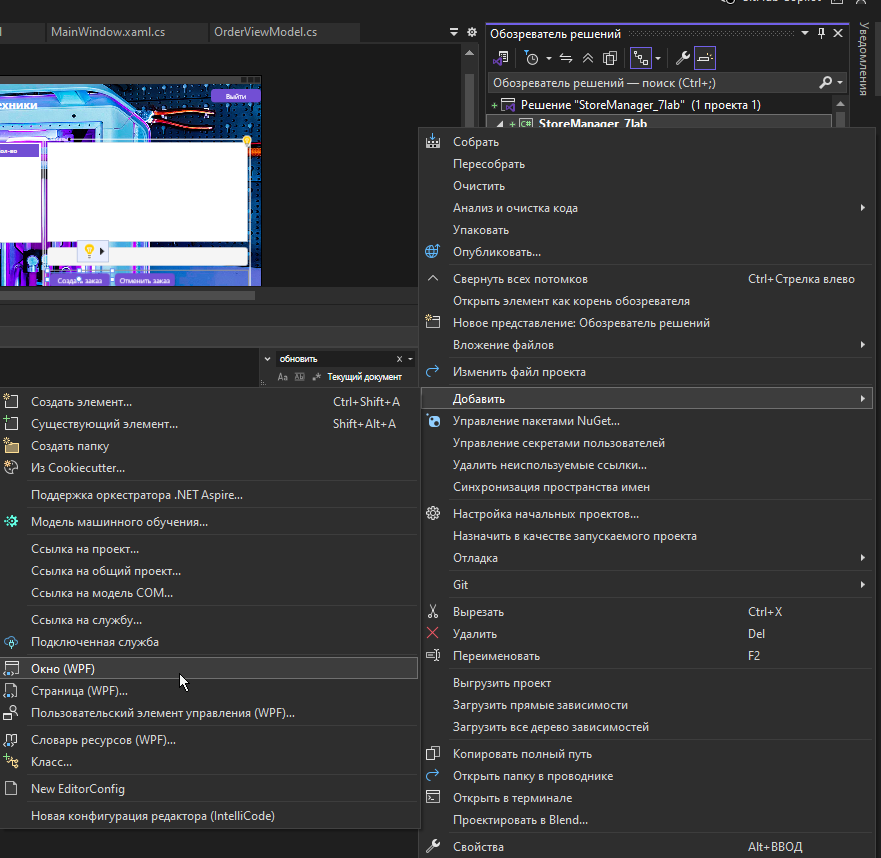
\includegraphics[width=0.8\textwidth]{fig/1}
	\caption{Добавление нового окна в приложение}
	% \label{fig:add_new_window}
\end{figure}

\noindent В листинге~\ref{lst:login_form_markup} приведен пример разметки для окна входа пользователя (логина).

\begin{code}
	\begin{minted}{xml}
 <StackPanel Margin="30" VerticalAlignment="Center">
        <TextBlock Text="Вход"
                   FontSize="24"
                   FontWeight="Bold"
                   HorizontalAlignment="Center"
                   Margin="0,0,0,20" />

        <TextBlock Text="Логин:" FontWeight="SemiBold"/>
        <TextBox Text="{Binding Username}" Margin="0,5,0,5" Padding="5"/>

        <TextBlock Text="Пароль:" FontWeight="SemiBold"/>
        <PasswordBox x:Name="PasswordBox"
                     
                     Margin="0,5,0,10"
                     Padding="5"
                     PasswordChanged="PasswordBox_PasswordChanged"/>

        <Button Content="Войти"
        Style="{StaticResource PurpleButton}"
        Command="{Binding LoginCommand}" />


        <!-- Ссылка на регистрацию -->
        <TextBlock HorizontalAlignment="Left" FontSize="12">
            <Run Text="Нет аккаунта? "/>
            <Run Text="Регистрация"
                 
                 Foreground="#8703ab"
                 TextDecorations="Underline"
                 Cursor="Hand"
                 MouseDown="RegisterText_MouseDown"/>
        </TextBlock>
</StackPanel> 
\end{minted}
	\caption{Разметка формы входа (\colorGIT{\href{https://github.com/WebMasterIT/Csharp_Labs/blob/main/7_lab_WPF/StoreManager_7lab/StoreManager_7lab/LoginWindow.xaml}{\texttt{LoginWindow.xaml}}})}
	\label{lst:login_form_markup}
\end{code}

\noindent Затем необходимо добавить следующий листинг в \texttt{LoginWindow.xaml.cs} (листинг~\ref{lst:login_window_cs}).
\begin{code}
	\begin{minted}{csharp}
namespace StoreManager_7lab
{

    public partial class LoginWindow : Window
    {
        private void RegisterText_MouseDown(object sender, MouseButtonEventArgs e)
        {
            var reg = new RegisterWindow();
            reg.ShowDialog();
             
            this.Close();
        }
        public LoginWindow()
        {
            InitializeComponent();
            if (DataContext is LoginViewModel vm)
            {
                vm.LoginSucceeded += () => this.Close();
            }
        }   

        private void PasswordBox_PasswordChanged(object sender, RoutedEventArgs e)
        {
            if (DataContext is LoginViewModel vm)
                vm.Password = PasswordBox.Password;
        }
    }
}
\end{minted}
	\caption{\colorGIT{\href{https://github.com/WebMasterIT/Csharp_Labs/blob/main/7_lab_WPF/StoreManager_7lab/StoreManager_7lab/RegisterWindow.xaml.cs}{\texttt{LoginWindow.xaml.cs}}}}
	\label{lst:login_window_cs}
\end{code}

В данном листинге (см. листинг~\ref{lst:login_form_markup}) учитывается, что после входа пользователя в приложение данная форма будет закрыта, а также есть возможность открыть окно регистрации по ссылке, нажав на соответствующий текст в форме.
Далее будет рассмотрено создание формы регистрации пользователей. В данном случае для этого был создан файл \texttt{RegisterWindow.xaml}.
Пример разметки для формы регистрации приведен в листинге~\ref{lst:register_form_markup}.

\begin{code}
	\begin{minted}{xml}
<Window x:Class="StoreManager_7lab.RegisterWindow"
        xmlns="http://schemas.microsoft.com/winfx/2006/xaml/presentation"
        xmlns:x="http://schemas.microsoft.com/winfx/2006/xaml"
        Title="Регистрация"> <!-- Added Window tag for completeness -->
    <Grid Margin="30">
        <Grid.RowDefinitions>
            <RowDefinition Height="Auto"/>
            <RowDefinition Height="Auto"/>
            <RowDefinition Height="Auto"/>
            <RowDefinition Height="Auto"/>
            <RowDefinition Height="Auto"/>
            <RowDefinition Height="*"/>
        </Grid.RowDefinitions>

        <TextBlock Grid.Row="0"
                   Text="Регистрация"
                   FontSize="24"
                   FontWeight="Bold"
                   HorizontalAlignment="Center"
                   Margin="0,0,0,20"
                   Foreground="#8703ab"/>

        <TextBlock Grid.Row="1" Text="Имя пользователя:"/>
        <TextBox Grid.Row="2"
                 Margin="0,5,0,10"
                 Padding="3"
                 Text="{Binding Username, UpdateSourceTrigger=PropertyChanged}"
                 Background="#2A2A2A"
                 BorderBrush="#8703ab"
                 Foreground="White" />

        <TextBlock Grid.Row="3" Text="Пароль:"/>
        <PasswordBox Grid.Row="4"
                     Margin="0,5,0,10"
                     x:Name="PasswordBox"
                     Padding="3"
                     PasswordChanged="PasswordBox_PasswordChanged"
                     Background="#2A2A2A"
                     BorderBrush="#8703ab"
                     Foreground="White"/>

        <StackPanel Grid.Row="5" Orientation="Vertical">
            <ComboBox ItemsSource="{Binding Roles}"
                      SelectedItem="{Binding SelectedRole}"  
                      Foreground="#8703ab"
                      Margin="0,0,0,10"/>

            <!-- Ссылка на вход -->
            <TextBlock HorizontalAlignment="Left" FontSize="12">
                 <Run Text="Уже зарегистриованы? "/>
                 <Run Text="Войти"
                      Foreground="#8703ab"
                      TextDecorations="Underline"
                      Cursor="Hand"
                      MouseDown="RegisterText_MouseDown"/> <!-- Assumed this is for LoginText_MouseDown -->
            </TextBlock>

            <Button Content="Зарегистрироваться"
                    Command="{Binding RegisterCommand}"
                    Background="#8703ab"
                    Foreground="White"
                    FontWeight="Bold"
                    Height="35"/>
        </StackPanel>
    </Grid>
</Window>
\end{minted}
	\caption{Разметка окна регистрации (\colorGIT{\href{https://github.com/WebMasterIT/Csharp_Labs/blob/main/7_lab_WPF/StoreManager_7lab/StoreManager_7lab/RegisterWindow.xaml}{\texttt{RegisterWindow.xaml}}})}
	\label{lst:register_form_markup}
\end{code}

Далее необходимо реализовать методы, отвечающие за функционирование кнопок самой формы (листинг~\ref{lst:register_window_cs}).
\begin{code}
	\begin{minted}{csharp}
namespace StoreManager_7lab
{
    public partial class RegisterWindow : Window
    {
        public RegisterWindow()
        {
            InitializeComponent();

            if (DataContext is RegisterViewModel vm)
            {
                vm.RegistrationSucceeded += OnRegistrationSucceeded;
            }
        }

        private void PasswordBox_PasswordChanged(object sender, RoutedEventArgs e)
        {
            if (DataContext is RegisterViewModel vm)
            {
                vm.Password = ((PasswordBox)sender).Password;
            }
        }
        // Changed from RegisterText_MouseDown to LoginText_MouseDown based on context
        private void LoginText_MouseDown(object sender, MouseButtonEventArgs e) 
        {
            var loginWindow = new LoginWindow();
            loginWindow.Show();

            this.Close(); // закрываем текущее окно регистрации
        }
        private void OnRegistrationSucceeded()
        {
            Application.Current.Dispatcher.Invoke(() =>
            {
                // Show success message window before login window
                var successWindow = new SuccessWindow();
                successWindow.ShowDialog();

                var loginWindow = new LoginWindow();
                loginWindow.Show();
                this.Close();
            });
        }
    }
}
\end{minted}
	\caption{Методы формы регистрации (\colorGIT{\href{https://github.com/WebMasterIT/Csharp_Labs/blob/main/7_lab_WPF/StoreManager_7lab/StoreManager_7lab/RegisterWindow.xaml.cs}{\texttt{RegisterWindow.xaml.cs}}})}
	\label{lst:register_window_cs}
\end{code}

Также можно добавить пользовательский вариант окна уведомления об успешной регистрации пользователя.
Необходимо добавить новое окно и назвать его \texttt{SuccessWindow.xaml}.
В листинге~\ref{lst:success_window_markup} приведена разметка данного окна.

\begin{code}
	\begin{minted}{xml}
<Window x:Class="StoreManager_7lab.SuccessWindow"
        xmlns="http://schemas.microsoft.com/winfx/2006/xaml/presentation"
        xmlns:x="http://schemas.microsoft.com/winfx/2006/xaml"
        Title="Успех"
        Height="150" Width="300"
        WindowStartupLocation="CenterScreen"
        Background="#8703ab">
    <Grid>
        <TextBlock Text="Регистрация успешна!"
                   Foreground="White"
                   FontSize="18"
                   FontWeight="Bold"
                   HorizontalAlignment="Center"
                   VerticalAlignment="Center"/>
        <!-- Removed OkButton_Click as it is not in the XAML -->
    </Grid>
</Window>
\end{minted}
	\caption{Разметка окна успешной регистрации (\colorGIT{\href{https://github.com/WebMasterIT/Csharp_Labs/blob/main/7_lab_WPF/StoreManager_7lab/StoreManager_7lab/SuccessWindow.xaml}{\texttt{SuccessWindow.xaml}}})}
	\label{lst:success_window_markup}
\end{code}

\begin{code}
	\begin{minted}{csharp}
namespace StoreManager_7lab
{
    public partial class SuccessWindow : Window
    {
        public SuccessWindow()
        {
            InitializeComponent();
            // Example: Close after a delay or add a button programmatically
            // For simplicity, this window might close itself or be closed by parent logic
        }

        // This method was in the original text but no button was in XAML.
        // If a button is added, its Click event can be wired here.
        // private void OkButton_Click(object sender, RoutedEventArgs e)
        // {
        //     this.Close();
        // }
    }
}
\end{minted}
	\caption{\colorGIT{\href{https://github.com/WebMasterIT/Csharp_Labs/blob/main/7_lab_WPF/StoreManager_7lab/StoreManager_7lab/SuccessWindow.xaml.cs}{\texttt{SuccessWindow.xaml.cs}}}}
	% \label{lst:success_window_cs}
\end{code}

\newpage

\section{DTO (Data Transfer Object)}
DTO (Data Transfer Object) — это объект, предназначенный для передачи данных между слоями приложения или между клиентом и сервером. В контексте Web API DTO особенно полезны для отделения внутренней модели базы данных от той, что используется внешними клиентами (например, WPF или другим API-клиентом).

\subsection{Зачем нужны DTO?}
\begin{itemize}
	\item \textbf{Изоляция модели базы данных:} DTO позволяет не раскрывать клиенту внутреннюю структуру сущностей, связанных с БД. Это снижает риск случайного или преднамеренного изменения чувствительных данных.
	\item \textbf{Упрощение данных:} Иногда внутренние модели содержат навигационные свойства, связанные сущности и прочее — всё это не всегда нужно на клиенте. DTO может содержать только необходимую информацию.
	\item \textbf{Валидация и контроль:} DTO позволяет настроить отдельные правила валидации, которые могут отличаться от ограничений модели БД.
	\item \textbf{Безопасность:} DTO защищает от уязвимостей, когда злоумышленник может отправить больше данных, чем нужно (например, роль пользователя в User, которую нельзя задавать напрямую через API без проверки).
\end{itemize}
Далее будут рассмотрены DTO, применяемые в данной лабораторной для входа и регистрации пользователей.

\noindent \textbf{Пример 1: \texttt{LoginDto:}}
\begin{minted}{csharp}
namespace StoreManagerApi.Models
{
    public class LoginDto
    {
        public string Username { get; set; } // Логин пользователя
        public string Password { get; set; } // Пароль
    }
}
\end{minted}
\texttt{LoginDto} используется только для входа в систему. Не содержит Id, Role или других свойств, которые есть в полной модели User. Это делает передачу данных более безопасной и упрощённой.

\noindent \textbf{Пример 2: \texttt{UserRegisterDto} (если бы он был)}
\begin{minted}{csharp}
public class UserRegisterDto
{
    public string Username { get; set; }
    public string Password { get; set; }
    public string Role { get; set; } // Добавлено для регистрации, если роль передается
}
\end{minted}
\texttt{UserRegisterDto} используется для регистрации. Он позволяет задать имя, пароль и роль, не включая другие свойства модели User, такие как Id, который создаётся автоматически.

\noindent \textbf{Почему не стоит использовать саму модель User:}
\begin{itemize}
	\item Она может содержать больше данных, чем нужно;
	\item Она может подвергаться сериализации/десериализации, что может открыть доступ к Role или Id;
	\item Это нарушает принцип единой ответственности: DTO отвечает только за передачу конкретных данных.
\end{itemize}

\newpage

\section{Контроллер регистрации}
Для реализации данного контроллера необходимо в приложении ASP.NET в папке \texttt{Controllers} создать файл \texttt{AuthController.cs}.
Данный контроллер отвечает за:
\begin{enumerate}
	\item Регистрацию пользователей (POST \texttt{/api/auth/register});
	\item Получение всех пользователей (служебный метод — GET \texttt{/api/auth/all});
	\item Аутентификацию (логин) с выдачей JWT-токена (POST \texttt{/api/auth/login}).
\end{enumerate}
Он работает совместно с Entity Framework Core (через \texttt{StoreDbContext}) и системой JWT-аутент\-ификации.

\subsection{JWT (JSON Web Token)}
JWT — это стандарт для безопасной передачи данных между двумя сторонами как JSON-объект. Он используется для авторизации и передачи удостоверений пользователя. В ASP.NET Core JWT применяется для защиты API и проверки прав пользователя.
JWT состоит из трёх частей:
\begin{itemize}
	\item Header — указывает тип токена и алгоритм подписи (обычно HMAC SHA256).
	\item Payload — содержит данные (претензии), например имя пользователя, его роль.
	\item Signature — создаётся на основе header, payload и секретного ключа.
\end{itemize}
\textbf{Преимущества JWT:}
\begin{enumerate}
	\item Без состояния (stateless).
	\item Передаётся через заголовки HTTP (Authorization: Bearer).
	\item Подписан и проверяется на подлинность.
\end{enumerate}
\textbf{Как устроен JWT в этом коде?}
\begin{enumerate}
	\item JWT формируется вручную в методе Login:
	\item Находится пользователь по имени и паролю;
	\item Формируется список претензий (claims) — имя и роль;
	\item Создаётся симметричный ключ с помощью \texttt{SymmetricSecurityKey};
	\item Подписывается токен с использованием HMAC SHA256;
	\item Возвращается токен клиенту в формате JSON.
\end{enumerate}
Полный листинг данного контроллера рассмотрен в листинге~\ref{lst:auth_controller}.
\begin{code}
	\begin{minted}[fontsize = \fontsize{10}{11.5}]{csharp}
using Microsoft.AspNetCore.Mvc;
using Microsoft.EntityFrameworkCore; // Предполагается, что StoreDbContext здесь
using Microsoft.AspNetCore.Identity; // Для PasswordHasher
using System.Linq;
using System.Security.Claims;
using Microsoft.IdentityModel.Tokens;
using System.Text;
using System.IdentityModel.Tokens.Jwt;
using System; // Для DateTime
// Assuming StoreDbContext and User are defined elsewhere
// namespace StoreManagerApi.Data { public class StoreDbContext : DbContext { /* ... */ } }
// namespace StoreManagerApi.Models { public class User { /* ... */ } }
// namespace StoreManagerApi.Models { public class LoginDto { /* ... */ } }


[ApiController]
[Route("api/[controller]")]
public class AuthController : ControllerBase
{
    private readonly StoreDbContext _context; // StoreDbContext должен быть определен
    // private readonly UserManager<User> _userManager; // Если используется ASP.NET Core Identity
    // private readonly SignInManager<User> _signInManager; // Если используется ASP.NET Core Identity

    public AuthController(StoreDbContext context) // UserManager<User> userManager
    {
        _context = context;
        // _userManager = userManager;
    }

    // POST: api/auth/register
    // Регистрирует нового пользователя с хешированием пароля
    [HttpPost("register")]
    public IActionResult Register(User user) // User должен быть моделью с Username, Password, Role
    {
        // Проверка: если пользователь уже существует, вернуть ошибку
        if (_context.Users.Any(u => u.Username == user.Username))
            return BadRequest("Такой пользователь уже существует");

        var hasher = new PasswordHasher<User>();
        user.Password = hasher.HashPassword(user, user.Password); // Хешируем пароль

        _context.Users.Add(user); // Добавляем пользователя в БД
        _context.SaveChanges();   // Сохраняем изменения

        return Ok("Регистрация прошла успешно");
    }

    // GET: api/auth/all
    // Возвращает всех пользователей (можно использовать для теста)
    [HttpGet("all")]
    public IActionResult GetAllUsers()
    {
        return Ok(_context.Users.ToList()); // Возвращаем список всех пользователей
    }

    // POST: api/auth/login
    // Авторизация: проверка логина и пароля, выдача JWT-токена
    [HttpPost("login")]
    public IActionResult Login(LoginDto dto) // LoginDto должен быть определен
    {
        // Поиск пользователя по логину
        var user = _context.Users.FirstOrDefault(u => u.Username == dto.Username);
        if (user == null)
            return Unauthorized("Неверный логин");

        var hasher = new PasswordHasher<User>();
        // Сравнение введённого пароля с хешем из БД
        var result = hasher.VerifyHashedPassword(user, user.Password, dto.Password);

        if (result == PasswordVerificationResult.Failed)
            return Unauthorized("Неверный пароль");

        // Создание набора claims (утверждений) о пользователе
        var claims = new[]
        {
            new Claim(ClaimTypes.Name, user.Username), // Имя пользователя
            new Claim(ClaimTypes.Role, user.Role)      // Его роль (Admin/Customer)
        };

        // Генерация ключа и токена
        var key = new SymmetricSecurityKey(Encoding.UTF8.GetBytes("THIS_IS_MY_SUPER_SECRET_KEY_1234567890")); // Ключ должен быть безопасным и из конфигурации
        var creds = new SigningCredentials(key, SecurityAlgorithms.HmacSha256);

        var token = new JwtSecurityToken(
            claims: claims,
            expires: DateTime.Now.AddHours(2), // Время действия токена
            signingCredentials: creds);        // Подпись токена

        // Отправка токена клиенту
        return Ok(new
        {
            token = new JwtSecurityTokenHandler().WriteToken(token), // строка-токен
            role = user.Role // роль для клиента
        });
    }
}
\end{minted}
	\caption{Контроллер регистрации (\colorGIT{\href{https://github.com/WebMasterIT/Csharp_Labs/blob/2c848a1824368d20b0ec88782fee773cec93c32f/7lab_ASPNET/StoreManagerApi/Controllers/AuthController.cs}{\texttt{AuthController.cs}}})}
	\label{lst:auth_controller}
\end{code}

\noindent Далее будет рассмотрен поэтапно полный листинг контроллера регистрации.
\begin{minted}{csharp}
[ApiController]
[Route("api/[controller]")]
public class AuthController : ControllerBase
\end{minted}
\begin{itemize}
	\item Атрибут \texttt{ApiController} говорит ASP.NET, что это контроллер Web API;
	\item \texttt{Route("api/[controller]")} означает маршрут \texttt{api/auth}.
\end{itemize}
\begin{minted}{csharp}
private readonly StoreDbContext _context;
public AuthController(StoreDbContext context)
{
    _context = context;
}
\end{minted}
\begin{itemize}
	\item зависимость от базы данных внедряется через DI;
	\item используется контекст для чтения и записи пользователей.
\end{itemize}
Внедрение зависимости от базы данных через Dependency Injection (DI) означает, что объект \texttt{StoreDbContext} не создаётся вручную в каждом контроллере, а предоставляется автоматически системой ASP.NET Core.
Dependency Injection — это паттерн проектирования, при котором зависимости (например, классы, которые нужны контроллеру) передаются извне, а не создаются внутри класса.
В контексте ASP.NET Core:
\begin{itemize}
	\item \texttt{StoreDbContext} зарегистрирован как сервис в методе \texttt{builder.Services.AddDbContext<StoreDb\-Context>()} в \texttt{Program.cs}.
	\item когда создаётся экземпляр контроллера \texttt{AuthController}, ASP.NET Core автоматически передаёт туда экземпляр \texttt{StoreDbContext}.
\end{itemize}

\noindent \textbf{Метод регистрации}
\begin{minted}{csharp}
[HttpPost("register")]
public IActionResult Register(User user)
{
    // Проверка: если пользователь уже существует, вернуть ошибку
    if (_context.Users.Any(u => u.Username == user.Username))
        return BadRequest("Такой пользователь уже существует");

    var hasher = new PasswordHasher<User>();
    user.Password = hasher.HashPassword(user, user.Password); // Хешируем пароль

    _context.Users.Add(user); // Добавляем пользователя в БД
    _context.SaveChanges();   // Сохраняем изменения

    return Ok("Регистрация прошла успешно");
}
\end{minted}
\begin{itemize}
	\item проверяет, существует ли уже пользователь;
	\item добавляет нового в базу данных;
	\item возвращает 200 OK, если всё прошло успешно.
\end{itemize}
Этот код усиливает безопасность системы авторизации, добавляя хеширование паролей с использованием стандартного компонента ASP.NET Core — \texttt{PasswordHasher<T>}.
Вместо того чтобы хранить пароли в базе данных в виде обычного текста (что крайне небезопасно), при регистрации пароль пользователя преобразуется в хеш, и только он сохраняется. При логине введённый пароль сравнивается с сохранённым хешем — если они совпадают, пользователь считается аутентифицированным.

\noindent \textbf{Регистрация с хешированием:}
\begin{minted}{csharp}
var hasher = new PasswordHasher<User>();
user.Password = hasher.HashPassword(user, user.Password);
\end{minted}
\begin{itemize}
	\item \texttt{PasswordHasher<User>} — встроенный класс, который реализует надёжный алгоритм хеширования.
	\item \texttt{HashPassword()} — создаёт уникальный хеш для пароля. Даже одинаковые пароли разных пользователей будут иметь разные хеши.
\end{itemize}
После этого хеш сохраняется в базу вместо самого пароля.

\noindent \textbf{Авторизация и проверка хеша:}
\begin{minted}{csharp}
var user = _context.Users.FirstOrDefault(u => u.Username == dto.Username);
if (user == null)
    return Unauthorized ("Неверный логин");

var hasher = new PasswordHasher<User>();
var result = hasher.VerifyHashedPassword(user, user.Password, dto.Password);
if (result == PasswordVerificationResult.Failed)
    return Unauthorized ("Неверный пароль");
\end{minted}
\begin{itemize}
	\item \texttt{VerifyHashedPassword()} проверяет, совпадает ли хеш из БД с паролем, введённым пользователем.
	\item Метод возвращает \texttt{Success}, \texttt{Failed} или \texttt{SuccessRehashNeeded}.
\end{itemize}

\noindent \textbf{Получение всех пользователей}
\begin{minted}{csharp}
[HttpGet("all")]
public IActionResult GetAllUsers()
{
    return Ok(_context.Users.ToList());
}
\end{minted}
\begin{itemize}
	\item возвращает список всех зарегистрированных пользователей;
	\item полезен только для отладки. Не должен быть открыт в боевом API.
\end{itemize}

\noindent \textbf{Метод входа (\texttt{Login})}
\begin{minted}{csharp}
[HttpPost("login")]
public IActionResult Login(LoginDto dto)
{
    var user = _context.Users.FirstOrDefault(u => u.Username == dto.Username); // Пароль проверяется ниже с хешем
    if (user == null)
        return Unauthorized("Неверный логин или пароль"); // Общее сообщение
    // ... (проверка хеша пароля как выше) ...
\end{minted}
\begin{itemize}
	\item проверка имени пользователя и пароля (с хешем);
	\item если не найден: ошибка 401 Unauthorized.
\end{itemize}
\begin{minted}{csharp}
var hasher = new PasswordHasher<User>();
// Сравнение введённого пароля с хешем из БД
var result = hasher.VerifyHashedPassword(user, user.Password, dto.Password);
if (result == PasswordVerificationResult.Failed)
    return Unauthorized("Неверный пароль");

var claims = new[]
{
    new Claim(ClaimTypes.Name, user.Username),
    new Claim(ClaimTypes.Role, user.Role)
};
\end{minted}
Формирование претензий (Claims) — имя и роль пользователя.
Claims (утверждения) — это пары ключ-значение, которые представляют информацию о пользователе или субъекте токена. Они встраиваются в Payload JWT-токена и используются системой аутентификации и авторизации для принятия решений о доступе.
\begin{minted}{csharp}
var key = new SymmetricSecurityKey(Encoding.UTF8.GetBytes("THIS_IS_MY_SUPER_SECRET_KEY_1234567890"));
var creds = new SigningCredentials(key, SecurityAlgorithms.HmacSha256);
\end{minted}
Создаётся ключ шифрования и подпись токена.
\begin{minted}{csharp}
var token = new JwtSecurityToken(
    claims: claims,
    expires: DateTime.Now.AddHours(2),
    signingCredentials: creds);
\end{minted}
Собирается сам токен: данные + срок действия + подпись.
\begin{minted}{csharp}
    return Ok(new
    {
        token = new JwtSecurityTokenHandler().WriteToken(token),
        role = user.Role
    });
} // Закрытие метода Login
\end{minted}
Возвращается JSON с токеном и ролью пользователя;
Этот токен потом передаётся в заголовке \texttt{Authorization: Bearer}.

\noindent \textbf{Пример успешного ответа}
\begin{minted}{json}
{
  "token": "eyJhbGciOiJIUzI1NiIsInR5cCI6...",
  "role": "Admin"
}
\end{minted}

\newpage

\section{Реализация ViewModel для формы регистрации}
Класс \texttt{RegisterViewModel} реализует интерфейс \texttt{INotifyPropertyChanged} и выступает как ViewModel для формы регистрации (например, \texttt{RegisterWindow.xaml}).
Он содержит свойства, связанные с вводом (логин, пароль, роль), команды, вызываемые кнопками, и методы взаимодействия с API через \texttt{ApiService}.
Реализация ViewModel для проекта WPF представлена в листинге~\ref{lst:register_view_model}.

\begin{code}
	\begin{minted}{csharp}
using System;
using System.Collections.ObjectModel;
using System.ComponentModel;
using System.Runtime.CompilerServices;
using System.Threading.Tasks;
using System.Windows;
using System.Windows.Input;
// Предполагается наличие RelayCommand, ApiService, UserRegisterDto, SuccessWindow, LoginWindow

public class RegisterViewModel : INotifyPropertyChanged
{
    // Поля, связанные с пользовательским вводом
    private string _username;
    public string Username
    {
        get => _username;
        set { _username = value; OnPropertyChanged(); ((RelayCommand)RegisterCommand).RaiseCanExecuteChanged(); }
    }

    private string _password;
    public string Password
    {
        get => _password;
        set { _password = value; OnPropertyChanged(); ((RelayCommand)RegisterCommand).RaiseCanExecuteChanged(); }
    }

    public ObservableCollection<string> Roles { get; } = new() { "Customer", "Admin" };

    private string _selectedRole;
    public string SelectedRole
    {
        get => _selectedRole;
        set { _selectedRole = value; OnPropertyChanged(); ((RelayCommand)RegisterCommand).RaiseCanExecuteChanged(); }
    }

    public ICommand RegisterCommand { get; }             // Команда регистрации (привязана к кнопке)

    public event Action RegistrationSucceeded;           // Событие, вызываемое при успешной регистрации

    private readonly ApiService _api = new ApiService(); // Сервис взаимодействия с Web API

    // Конструктор ViewModel
    public RegisterViewModel()
    {
        // Привязка команды к методу регистрации и условию доступности
        RegisterCommand = new RelayCommand(
            async _ => await RegisterAsync(),
            _ => CanRegister());
    }
    // Асинхронный метод регистрации пользователя
    private async Task RegisterAsync()
    {
        try
        {
            // await _api.InitAsync(); // (необязательная инициализация клиента, если есть)

            // Создание DTO с введёнными данными
            var dto = new UserRegisterDto // UserRegisterDto должен быть определен
            {
                Username = Username,
                Password = Password,
                Role = SelectedRole
            };

            await _api.RegisterAsync(dto); // Отправка на сервер

            // Вызов события для закрытия окна и открытия окна входа из кода RegisterWindow.xaml.cs
            RegistrationSucceeded?.Invoke();
            
            // Закрытие текущего окна регистрации (это может быть сделано в обработчике RegistrationSucceeded)
            // foreach (Window window in Application.Current.Windows)
            // {
            //     if (window is RegisterWindow) // RegisterWindow должен быть определен
            //     {
            //         window.Close();
            //         break;
            //     }
            // }
        }
        catch (Exception ex)
        {
            // Сообщение об ошибке
            MessageBox.Show($"Ошибка регистрации: {ex.Message}");
        }
    }
    // Условие для активации кнопки регистрации
    private bool CanRegister() =>
        !string.IsNullOrWhiteSpace(Username) &&
        !string.IsNullOrWhiteSpace(Password) &&
        !string.IsNullOrWhiteSpace(SelectedRole);

    // Реализация интерфейса INotifyPropertyChanged
    public event PropertyChangedEventHandler PropertyChanged;
    protected void OnPropertyChanged([CallerMemberName] string name = null) =>
        PropertyChanged?.Invoke(this, new PropertyChangedEventArgs(name));
}
\end{minted}
	\captionof{listing}{Класс \colorGIT{\href{https://github.com/WebMasterIT/Csharp_Labs/blob/main/7_lab_WPF/StoreManager_7lab/StoreManager_7lab/RegisterWindow.xaml.cs}{\texttt{RegisterViewModel}}}}
	\label{lst:register_view_model}
\end{code}

% \noindent \textbf{Описание методов листинга~\ref{lst:register_view_model}:}
\begin{enumerate}
	\item \textbf{\texttt{RegisterAsync()}}
	      Метод \texttt{RegisterAsync()} реализует основной алгоритм регистрации пользователя:
	      \begin{enumerate}
		      \item Выполняется предварительная инициализация API-сервиса через вызов \texttt{InitAsync()} (если такой метод есть и он необходим).
		      \item Создаётся объект \texttt{UserRegisterDto}, содержащий данные, введённые пользователем: имя, пароль и выбранную роль.
		      \item С помощью метода \texttt{\_api.RegisterAsync(dto)} данные отправляются на сервер в формате JSON, где происходит регистрация нового пользователя.
		      \item При успешной регистрации вызывается событие \texttt{RegistrationSucceeded}. В обработчике этого события (в \texttt{RegisterWindow.xaml.cs}) отображается окно подтверждения (\texttt{Success\-Window}), после чего запускается окно входа (\texttt{LoginWindow}).
		      \item Активное окно регистрации (\texttt{RegisterWindow}) закрывается (также в обработчике события).
	      \end{enumerate}
	      Метод обёрнут в конструкцию \texttt{try-catch}, обеспечивающую обработку исключений и отображение ошибок в форме диалогового окна.

	\item \textbf{\texttt{CanRegister()}}
	      \texttt{CanRegister()} определяет, можно ли активировать кнопку регистрации. Возвращает \texttt{true}, если все три поля (имя пользователя, пароль и роль) не пустые и не содержат только пробелы. В противном случае — \texttt{false}. Это предотвращает отправку неполных данных на сервер.

	\item \textbf{Метод \texttt{OnPropertyChanged(string name)}}
	      \texttt{OnPropertyChanged()} — вспомогательный метод, реализующий механизм уведомления об изменении свойств, требуемый интерфейсом \texttt{INotify\-Property\-Changed}. Он используется для обновления интерфейса в режиме реального времени при изменении свойств ViewModel.
\end{enumerate}

\section{Контроллер OrderController}
Контроллер \texttt{OrderController} — это важнейший компонент API, который управляет заказами в системе. Без него невозможно:
\begin{enumerate}
	\item Получить список заказов.
	\item Создать новый заказ.
	\item Удалить заказ (при наличии соответствующих прав).
\end{enumerate}
Он работает как интерфейс между клиентом (например, WPF-приложением) и базой данных, обрабатывая HTTP-запросы, выполняя валидацию данных и обеспечивая безопасность.

\noindent \textbf{Ключевая часть:}
\begin{minted}{csharp}
[Authorize(Roles = "Admin")] // Требует авторизации и роли Admin
[HttpDelete("{id}")]
public async Task<IActionResult> DeleteOrder(int id)
{
    // ... логика удаления ...
}
\end{minted}
Эти атрибуты обозначают, что данный метод удаления заказа:
\begin{itemize}
	\item требует авторизации (\texttt{[Authorize]});
	\item допускает доступ только пользователю с ролью Admin (\texttt{Roles = Admin});
	\item будет вызван по маршруту DELETE \texttt{/api/order/{id}} (например, \texttt{/api/order/5}).
\end{itemize}
Таким образом, безопасность обеспечивается на уровне маршрута: обычный пользователь не сможет удалить заказ, даже если знает правильный адрес.

\noindent \textbf{Основной код:}
\begin{minted}{csharp}
var order = await _context.Orders
    .Include(o => o.Items) // Включаем связанные элементы заказа
    .FirstOrDefaultAsync(o => o.Id == id);
\end{minted}
В данном случае:
\begin{itemize}
	\item \texttt{\_context.Orders} — обращение к таблице заказов;
	\item \texttt{.Include(o => o.Items)} — указывает EF Core, что нужно включить связанные записи из таблицы \texttt{OrderItems} (позиции заказа). Без этого \texttt{Items} будут \texttt{null};
	\item \texttt{.FirstOrDefaultAsync(o => o.Id == id)} — ищет первый заказ, чей Id совпадает с переданным. Если заказ не найден — вернёт \texttt{null}.
\end{itemize}
Затем выполняется проверка:
\begin{minted}{csharp}
if (order == null)
    return NotFound(); // Код 404, если заказ не найден
\end{minted}
Если заказ не найден — возвращается код ответа 404 Not Found.
Удаление заказа осуществляется с помощью метода \texttt{Remove}: \texttt{\_context.Orders.Remove(order);}
\begin{minted}{csharp}
await _context.SaveChangesAsync(); // Сохранение изменений в БД
\end{minted}
Сначала EF помечает объект как удалённый, а затем сохраняет изменения в базе. Благодаря каскадной настройке в DbContext, также удаляются связанные \texttt{OrderItem}.

\newpage

\section{Реализация ProductController}
\texttt{ProductController} — контроллер, отвечающий за управление товарами в API. Он реализует CRUD-операции для ресурса \texttt{Product}, а также демонстрирует работу с авторизацией на основе ролей.
Основные возможности \texttt{ProductController}:
\begin{enumerate}
	\item Позволяет всем пользователям просматривать список товаров и отдельные товары по ID.
	\item Предоставляет администраторам (роль Admin) возможность добавлять, редактировать и удалять товары.
	\item Использует базу данных через \texttt{StoreDbContext}, внедрённый через Dependency Injection.
	\item Защищён с помощью атрибутов \texttt{[Authorize]} и \texttt{[AllowAnonymous]}.
\end{enumerate}
В листинге~\ref{lst:product_controller} приведен полный код данного контроллера с комментариями.
\begin{code}
	\begin{minted}{csharp}
using Microsoft.AspNetCore.Mvc;
using Microsoft.EntityFrameworkCore;
using System.Collections.Generic;
using System.Threading.Tasks;
using Microsoft.AspNetCore.Authorization; // Для атрибутов авторизации
// Предполагается, что Product и StoreDbContext определены
// namespace StoreManagerApi.Models { public class Product { /* ... */ } }

namespace StoreManagerApi.Controllers
{
    [ApiController]
    [Route("api/[controller]")] // Базовый маршрут: api/Product
    public class ProductController : ControllerBase
    {
        private readonly StoreDbContext _context;

        // Внедрение зависимости через конструктор
        public ProductController(StoreDbContext context) => _context = context;

        // =============================
        // GET: /api/Product
        // Возвращает список всех товаров
        // Доступен без авторизации
        // =============================
        [AllowAnonymous] // Разрешает доступ без токена
        [HttpGet]
        public async Task<ActionResult<IEnumerable<Product>>> GetAll() =>
            await _context.Products.ToListAsync();

        // =============================
        // GET: /api/Product/5
        // Получает один товар по его ID
        // Доступен без авторизации
        // =============================
        [AllowAnonymous]
        [HttpGet("{id}")]
        public async Task<ActionResult<Product>> Get(int id)
        {
            var product = await _context.Products.FindAsync(id);
            return product == null ? NotFound() : Ok(product); // 404 если не найден
        }

        // =============================
        // POST: /api/Product
        // Создаёт новый товар
        // Только для роли Admin
        // =============================
        [Authorize(Roles = "Admin")] // Требует авторизации и роли Admin
        [HttpPost]
        public async Task<ActionResult<Product>> Create(Product product) // Возвращаем созданный продукт
        {
            _context.Products.Add(product);             // Добавляем в контекст
            await _context.SaveChangesAsync();          // Сохраняем изменения

            // Возвращаем статус 201 и маршрут к новому товару
            return CreatedAtAction(nameof(Get), new { id = product.Id }, product);
        }

        // =============================
        // PUT: /api/Product/5
        // Обновляет товар по ID
        // Только для роли Admin
        // =============================
        [Authorize(Roles = "Admin")]
        [HttpPut("{id}")]
        public async Task<IActionResult> Update(int id, Product product) // IActionResult, т.к. NoContent
        {
            if (id != product.Id) return BadRequest();  // Проверка ID

            _context.Entry(product).State = EntityState.Modified; // Помечаем как "изменённый"
            
            try
            {
                await _context.SaveChangesAsync(); // Сохраняем
            }
            catch (DbUpdateConcurrencyException)
            {
                if (!_context.Products.Any(e => e.Id == id)) // Проверяем, существует ли продукт
                {
                    return NotFound();
                }
                else
                {
                    throw;
                }
            }
            return NoContent(); // 204 — успешно, без тела
        }

        // =============================
        // DELETE: /api/Product/5
        // Удаляет товар по ID
        // Только для роли Admin
        // =============================
        [Authorize(Roles = "Admin")]
        [HttpDelete("{id}")]
        public async Task<IActionResult> Delete(int id) // IActionResult
        {
            var product = await _context.Products.FindAsync(id);
            if (product == null) return NotFound(); // 404 если не найден

            _context.Products.Remove(product);      // Удаление
            await _context.SaveChangesAsync();      // Сохраняем

            return NoContent(); // 204 — успешно удалено
        }
    }
}
\end{minted}
	\captionof{listing}{Контроллер \colorGIT{\href{https://github.com/WebMasterIT/Csharp_Labs/blob/main/7lab_ASPNET/StoreManagerApi/Controllers/ProductsController.cs}{\texttt{ProductController.cs}}}}
	\label{lst:product_controller}
\end{code}

\newpage

\section{ApiService}
Класс \texttt{ApiService} — это служба клиента WPF-приложения, которая взаимодействует с REST API (Web API на ASP.NET Core). Он отвечает за:
\begin{itemize}
	\item настройку подключения;
	\item авторизацию и хранение токена;
	\item выполнение CRUD-операций для товаров и заказов;
	\item регистрацию и логин пользователя.
\end{itemize}
Данный класс нужен, чтобы разгрузить ViewModel от сетевых вызовов и предоставить единый интерфейс для общения WPF-клиента с сервером. Это часть архитектуры MVVM.

\noindent \textbf{\iicon{} Пояснение с комментариями в коде:}
\begin{minted}{csharp}
// using System.Net.Http;
// using System.Net.Http.Headers; // For AuthenticationHeaderValue
// using System.Net.Http.Json; // For PostAsJsonAsync, ReadFromJsonAsync
// using System.Text.Json; // For JsonSerializer, JsonElement
// using System.Threading.Tasks;
// using System.Collections.Generic; // For List
// Models: Product, Order, UserRegisterDto must be defined

public class ApiService
{
    private HttpClient _http;        // Клиент для HTTP-запросов
    private string _token;           // JWT-токен, полученный при логине
    private string _role;            // Роль пользователя (Admin/Customer)
}
\end{minted}

\noindent \textbf{\iicon{} Инициализация клиента:}
\begin{minted}{csharp}
public async Task InitAsync() // Сделаем асинхронным, если TryUseHttps асинхронный
{
    var handler = new HttpClientHandler
    {
        // ВАЖНО: В реальном приложении используйте валидные сертификаты!
        ServerCertificateCustomValidationCallback = (message, cert, chain, errors) => true // Игнорируем SSL в dev
    };

    // Проверка: работает ли HTTPS?
    bool useHttps = await TryUseHttpsAsync();  // Назовем его Async

    // Настраиваем базовый адрес
    var baseUri = useHttps
        ? "https://localhost:7259/api/" // Порт HTTPS по умолчанию для ASP.NET Core
        : "http://localhost:5107/api/"; // Порт HTTP по умолчанию для ASP.NET Core

    _http = new HttpClient(handler)
    {
        BaseAddress = new Uri(baseUri)
    };
}

private async Task<bool> TryUseHttpsAsync() // Пример реализации
{
    try
    {
        using var testClient = new HttpClient(new HttpClientHandler { ServerCertificateCustomValidationCallback = (a,b,c,d) => true });
        testClient.Timeout = TimeSpan.FromSeconds(3); // Таймаут для проверки
        var response = await testClient.GetAsync("https://localhost:7259/api/Product"); // Пробный запрос
        return response.IsSuccessStatusCode;
    }
    catch
    {
        return false;
    }
}
\end{minted}
Метод \texttt{TryUseHttpsAsync()} пытается подключиться по HTTPS и возвращает \texttt{true}, если сервер отвечает.

\noindent \textbf{\iicon{} Работа с токеном:}
\begin{minted}{csharp}
public void SetToken(string token)
{
    _token = token;
    if (_http != null) // Убедимся, что HttpClient инициализирован
    {
        _http.DefaultRequestHeaders.Authorization = 
            new System.Net.Http.Headers.AuthenticationHeaderValue("Bearer", token); // Добавляем токен
    }
}

public void SetRole(string role) // Добавлен метод для установки роли
{
    _role = role;
}

public string GetRole() => _role; // Получение роли

public void ClearAuth() // Очистка авторизации
{
    _token = null;
    _role = null;
    if (_http != null)
    {
        _http.DefaultRequestHeaders.Authorization = null;
    }
}
\end{minted}
Также можно:
\begin{itemize}
	\item получить роль \texttt{GetRole()};
	\item очистить авторизацию \texttt{ClearAuth()} (удаляет токен из заголовков).
\end{itemize}

\noindent \textbf{\iicon{} Работа с продуктами (Product):}
\begin{minted}{csharp}
public async Task<List<Product>> GetProductsAsync()
{
    // HttpClient должен быть инициализирован через InitAsync()
    var response = await _http.GetAsync("Product"); 
    response.EnsureSuccessStatusCode(); // Проверка на ошибки HTTP
    var json = await response.Content.ReadAsStringAsync();

    // Опции десериализации для игнорирования регистра символов в именах свойств
    var options = new JsonSerializerOptions { PropertyNameCaseInsensitive = true };
    var products = JsonSerializer.Deserialize<List<Product>>(json, options);

    return products ?? new List<Product>();
}
\end{minted}
Также реализованы:
\begin{itemize}
	\item \texttt{AddProductAsync} — добавляет товар через POST \texttt{/api/Product};
	\item \texttt{UpdateProductAsync} — обновляет товар;
	\item \texttt{DeleteProductAsync} — удаляет товар.
\end{itemize}

\noindent \textbf{\iicon{󰄑} Работа с заказами (Order):}
\begin{minted}{csharp}
public async Task<List<Order>> GetOrdersAsync()
{
    if (string.IsNullOrWhiteSpace(_token)) return new List<Order>(); // Без токена нельзя

    var response = await _http.GetAsync("Order");
    if (response.StatusCode == System.Net.HttpStatusCode.Unauthorized) return new List<Order>();
    response.EnsureSuccessStatusCode();

    // Используем ReadFromJsonAsync для упрощения
    var orders = await response.Content.ReadFromJsonAsync<List<Order>>(
        new JsonSerializerOptions { PropertyNameCaseInsensitive = true });
    
    // Фильтрация для удаления null элементов если API может их вернуть
    return orders?.Where(o => o != null && o.Items != null).ToList() ?? new List<Order>();
}
\end{minted}
Также есть:
\begin{itemize}
	\item \texttt{AddOrderAsync(order)} — создание заказа;
	\item \texttt{DeleteOrderAsync(id)} — удаление по ID.
\end{itemize}

\noindent \textbf{\iicon{} Аутентификация и регистрация:}
\begin{minted}{csharp}
public async Task<bool> LoginAsync(string username, string password)
{
    var dto = new { Username = username, Password = password }; // Анонимный тип для LoginDto
    var response = await _http.PostAsJsonAsync("auth/login", dto);

    if (!response.IsSuccessStatusCode) return false;

    // Чтение JSON ответа для получения токена и роли
    var jsonDocument = await JsonDocument.ParseAsync(await response.Content.ReadAsStreamAsync());
    string token = jsonDocument.RootElement.GetProperty("token").GetString();
    string role = jsonDocument.RootElement.GetProperty("role").GetString();

    SetToken(token);
    SetRole(role); // Сохраняем роль

    return true;
}
\end{minted}
\textbf{Регистрация:}
\begin{minted}{csharp}
public async Task RegisterAsync(UserRegisterDto dto) // UserRegisterDto должен быть определен
{
    var options = new JsonSerializerOptions
    {
        PropertyNamingPolicy = null // Отключаем camelCase, если API ожидает PascalCase для DTO
    };

    var response = await _http.PostAsJsonAsync("auth/register", dto, options);
    response.EnsureSuccessStatusCode(); // Выбросит исключение при ошибке
}
\end{minted}

\newpage

\section{Program.cs}
Этот файл — это основная точка входа в ASP.NET Core Web API-приложение. Он находится в файле \texttt{Program.cs} и отвечает за настройку всех компонентов, сервисов, middleware, базы данных и запуск приложения. Ниже приведено его подробное описание и пояснение по блокам.
Этот файл конфигурирует:
\begin{itemize}
	\item регистрацию сервисов (DI);
	\item подключение базы данных через Entity Framework;
	\item настройку JWT-аутентификации;
	\item настройку CORS;
	\item генерацию Swagger-документации;
	\item запуск самого веб-сервера.
\end{itemize}
Полный \colorGIT{\href{https://github.com/WebMasterIT/Csharp_Labs/blob/main/7lab_ASPNET/StoreManagerApi/Program.cs}{листинг}} данного метода находится в репозитории \colorURL{\href{https://github.com/WebMasterIT/Csharp_Labs/tree/main}{GitHub} \iicon{}}.
Далее будет рассмотрена структура данного метода с комментариями.

\begin{code}
	\begin{minted}{csharp}
// using Microsoft.AspNetCore.Builder;
// using Microsoft.Extensions.DependencyInjection;
// using Microsoft.EntityFrameworkCore; // Для UseSqlite
// using Microsoft.AspNetCore.Authentication.JwtBearer; // Для AddJwtBearer
// using Microsoft.IdentityModel.Tokens; // Для TokenValidationParameters
// using System.Text; // Для Encoding
// using StoreManagerApi.Data; // Предполагаемый namespace для StoreDbContext

var builder = WebApplication.CreateBuilder(args); // Создаёт и конфигурирует приложение
\end{minted}
\end{code}

\noindent \textbf{\iicon{} Настройка JWT-аутентификации}
\begin{code}
	\begin{minted}{csharp}
builder.Services.AddAuthentication(options =>
{
    // Указываем, что по умолчанию используется схема JWT Bearer
    options.DefaultAuthenticateScheme = JwtBearerDefaults.AuthenticationScheme;
    options.DefaultChallengeScheme = JwtBearerDefaults.AuthenticationScheme;
})
.AddJwtBearer(options =>
{
    options.RequireHttpsMetadata = false; // Отключить HTTPS в режиме разработки (в production true)
    options.SaveToken = true;             // Сохранять токен в HttpContext после валидации
    options.TokenValidationParameters = new TokenValidationParameters
    {
        ValidateIssuer = false, // Не проверять издателя токена (true для production)
        ValidateAudience = false, // Не проверять получателя токена (true для production)
        ValidateLifetime = true, // Проверять срок действия токена
        ValidateIssuerSigningKey = true, // Проверять подпись токена
        IssuerSigningKey = new SymmetricSecurityKey( // Ключ должен совпадать с ключом генерации
            Encoding.UTF8.GetBytes("THIS_IS_MY_SUPER_SECRET_KEY_1234567890")) // Заменить на безопасный ключ из конфигурации!
        // ClockSkew = TimeSpan.Zero // Можно установить для точной проверки времени жизни
    };
});
\end{minted}
\end{code}
Этот блок необходим для правильной обработки токенов, выданных при логине.

\noindent \textbf{{\iicon{} Разрешение CORS}}
\begin{code}
	\begin{minted}{csharp}
builder.Services.AddCors(options =>
{
    options.AddPolicy("AllowAll", policy =>
    {
        policy.AllowAnyOrigin()  // Разрешить запросы с любого источника
              .AllowAnyHeader() // Разрешить любые заголовки
              .AllowAnyMethod(); // Разрешить любые HTTP-методы (GET, POST, etc.)
    });
});
\end{minted}
\end{code}
CORS нужен, если клиент (например, WPF, React) обращается к API с другого адреса.


\noindent \textbf{\iicon{󰆼} Настройка базы данных}
\begin{code}
	\begin{minted}{csharp}
builder.Services.AddDbContext<StoreDbContext>(options =>
    options.UseSqlite(builder.Configuration.GetConnectionString("DefaultConnection") 
                      ?? "Data Source=store.db")); // Подключение к SQLite, имя строки из appsettings.json
\end{minted}
\end{code}

Здесь подключается база данных и настраивается контекст \texttt{StoreDbContext} для Entity Framework Core.


\noindent \textbf{{\iicon{󰟾} Контроллеры и Swagger}}
\begin{code}
	\begin{minted}{csharp}
builder.Services.AddControllers()
    .AddJsonOptions(options =>
    {
        // Игнорировать циклические ссылки (например, Product -> OrderItem -> Product)
        options.JsonSerializerOptions.ReferenceHandler = System.Text.Json.Serialization.ReferenceHandler.IgnoreCycles;
        options.JsonSerializerOptions.PropertyNamingPolicy = null; // Если хотите PascalCase, а не camelCase
    });

builder.Services.AddEndpointsApiExplorer(); // Для генерации метаданных API
builder.Services.AddSwaggerGen();          // Для UI Swagger
\end{minted}
\end{code}

\noindent \textbf{\iicon{} Создание приложения и базы}
\begin{code}
	\begin{minted}[fontsize = \fontsize{10}{10}]{csharp}
var app = builder.Build();

// Создаёт базу данных при первом запуске, если она не существует
using (var scope = app.Services.CreateScope())
{
    var services = scope.ServiceProvider;
    try
    {
        var db = services.GetRequiredService<StoreDbContext>();
        db.Database.EnsureCreated(); // Создание БД, если ещё не создана
    }
    catch (Exception ex)
    {
        var logger = services.GetRequiredService<ILogger<Program>>();
        logger.LogError(ex, "An error occurred creating the DB.");
    }
}
\end{minted}
\end{code}

\noindent \textbf{{\iicon{} Middleware и запуск}}
\begin{code}
	\begin{minted}[fontsize = \fontsize{10}{10}]{csharp}
if (app.Environment.IsDevelopment())
{
    app.UseSwagger();    // Включаем Swagger только в режиме разработки
    app.UseSwaggerUI();  // Интерфейс документации Swagger
    app.UseDeveloperExceptionPage(); // Страница с деталями ошибок для разработчика
}

app.UseCors("AllowAll");             // Включаем CORS (политика "AllowAll")

// app.UseHttpsRedirection();        // Можно включить HTTPS, если настроен сертификат

app.UseRouting(); // Добавляем маршрутизацию (важно для порядка middleware)

app.UseAuthentication();            // Включаем аутентификацию JWT (проверяет токен)
app.UseAuthorization();             // Проверка авторизации и ролей (проверяет права доступа)

app.MapControllers();               // Маршрутизация контроллеров (api/...)

app.Run();                          // Запускает приложение
\end{minted}
\end{code}

\newpage

\section{Реализация интерфейса}
Далее необходимо рассмотреть реализацию интерфейса форм входа и регистрации, а также пользовательского интерфейса программы в зависимости от используемой роли. На рисунках~\ref{fig:login_form} – \ref{fig:register_form} приведен интерфейс форм входа (логина) и регистрации. На рисунке~\ref{fig:success_registration_window} приведен интерфейс окна с сообщением об успешной регистрации.

\begin{figure}[H]
	\centering
	\subfloat[Форма входа]{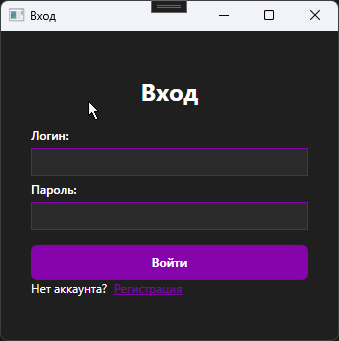
\includegraphics[width=0.45\textwidth]{fig/2} \label{fig:login_form}}
	\hfil
	\subfloat[Форма регистрации]{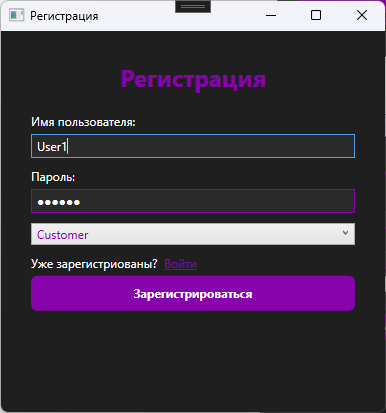
\includegraphics[width=0.45\textwidth]{fig/3} \label{fig:register_form}}
	\hfil
	\subfloat[Окно успешной регистрации]{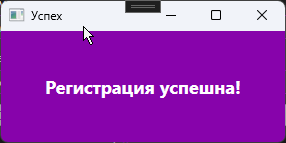
\includegraphics[width=0.45\textwidth]{fig/4} \label{fig:success_registration_window}}
	\caption{Реализация интерфейса входа и регистрации}
\end{figure}

В форме регистрации реализована возможность выбора роли: пользователь или администратор (Рисунок~\ref{fig:role_selection_registration}).
\begin{figure}[H]
	\centering
	[NONE]
	\caption{Выбор роли пользователя при регистрации}
	\label{fig:role_selection_registration}
\end{figure}

Интерфейс приложения для роли «Администратор» сохранил возможность добавления, удаления, обновления информации о товарах (Рисунок~\ref{fig:admin_interface}).

\begin{figure}[H]
	\centering
	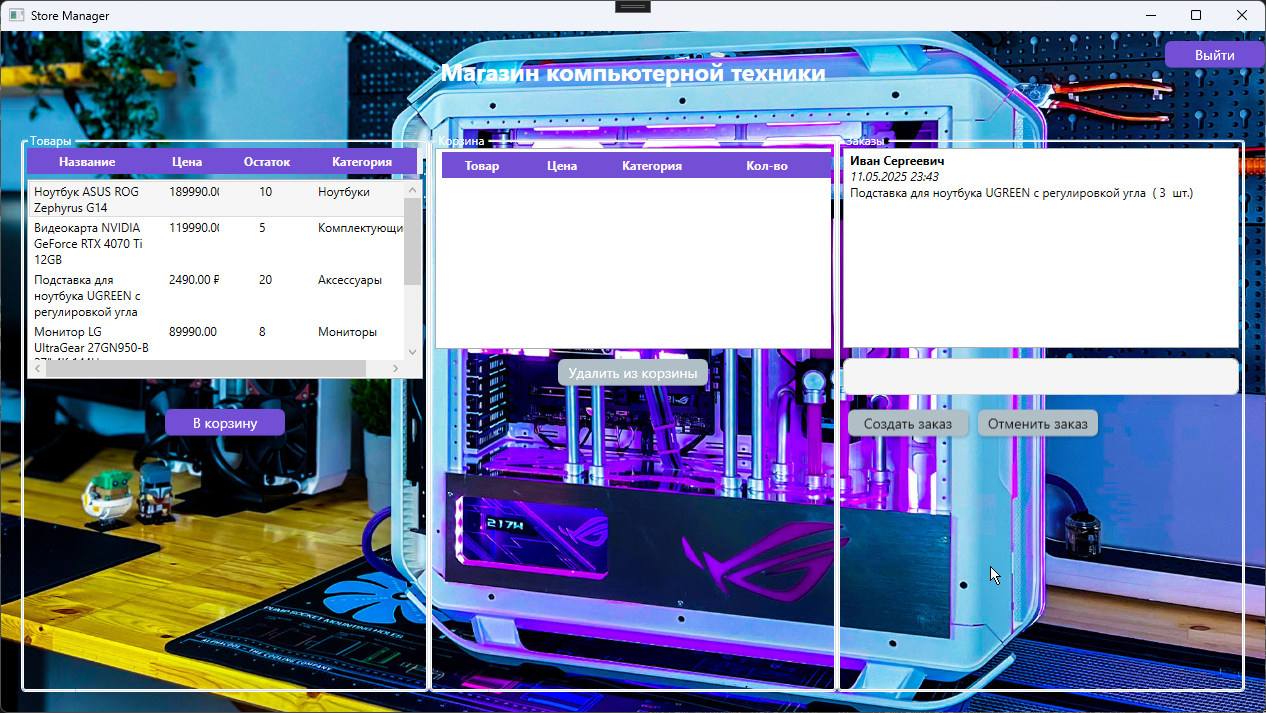
\includegraphics[width=0.8\textwidth]{fig/5.png}
	\caption{Интерфейс приложения для администратора}
	\label{fig:admin_interface}
\end{figure}

Интерфейс приложения для роли «Пользователь» (Рисунок~\ref{fig:user_interface}).
\begin{figure}[H]
	\centering
	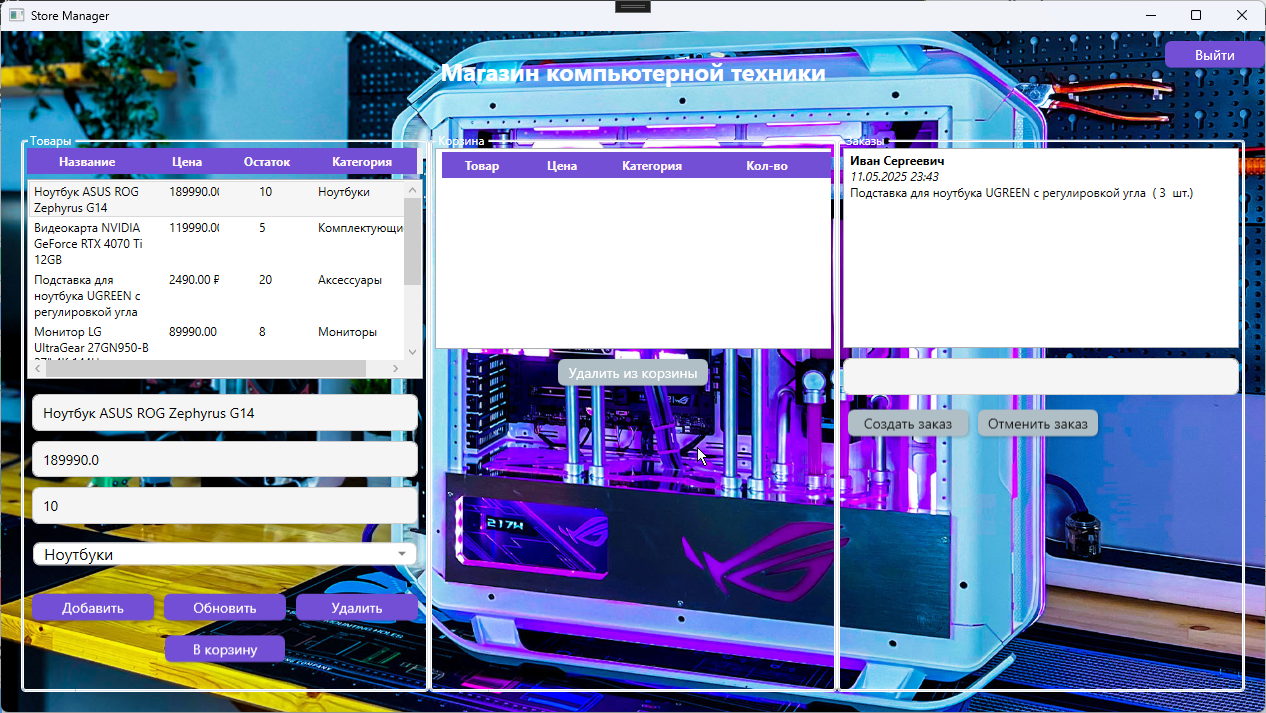
\includegraphics[width=0.8\textwidth]{fig/6.png}
	\caption{Интерфейс приложения для пользователя}
	\label{fig:user_interface}
\end{figure}

\newpage

\section{Вопросы по лабораторной работе №7}

\textbf{Аутентификация и регистрация}
\begin{enumerate}
	\item Как реализуется регистрация нового пользователя в системе?
	\item Почему важно хешировать пароль перед сохранением в базу данных?
	\item Как работает проверка пароля при входе?
	\item Что такое DTO и зачем они используются при регистрации и входе?
\end{enumerate}

\noindent \textbf{JWT и авторизация по ролям}
\begin{enumerate}
	\setcounter{enumi}{4} % Продолжаем нумерацию
	\item Как формируется JWT-токен при авторизации пользователя?
	\item Какие claims входят в JWT и для чего они используются?
	\item Как система определяет, имеет ли пользователь доступ к определённым действиям?
\end{enumerate}

\noindent \textbf{Архитектура и защита данных}
\begin{enumerate}
	\setcounter{enumi}{7}
	\item Почему нельзя использовать модель User напрямую в методе регистрации?
	\item В чём преимущества разделения моделей и DTO?
\end{enumerate}

\noindent \textbf{Клиентская часть (WPF)}
\begin{enumerate}
	\setcounter{enumi}{9}
	\item Как реализована форма входа и регистрации в WPF?
	\item Как определяется текущая роль пользователя в клиентском приложении?
	\item Чем отличается интерфейс пользователя и администратора?
\end{enumerate}

\noindent \textbf{MVVM и взаимодействие с API}
\begin{enumerate}
	\setcounter{enumi}{12}
	\item Как ViewModel взаимодействует с ApiService?
	\item Почему используется команда RegisterCommand в RegisterViewModel?
	\item Какие действия выполняет метод RegisterAsync()?
\end{enumerate}

\end{document}
